% !TeX root = ../dd.tex

\section{User Interface Design}
%  Provide an overview on how the user interface(s) of your system will
% look like; if you have included this part in the RASD, you can simply
% refer to what you have already done, possibly, providing here some
% extensions if applicable.

\subsection{Web and Mobile application}

The \emph{RASD} contains already several mockups of the mobile applications. In Fig. \ref{fig:ux_flowchart} we provide the flow diagrams describing the user experience of the client applications, which will be implemented by both the Mobile App and the Web App.

\begin{figure}[H]
    \centering
    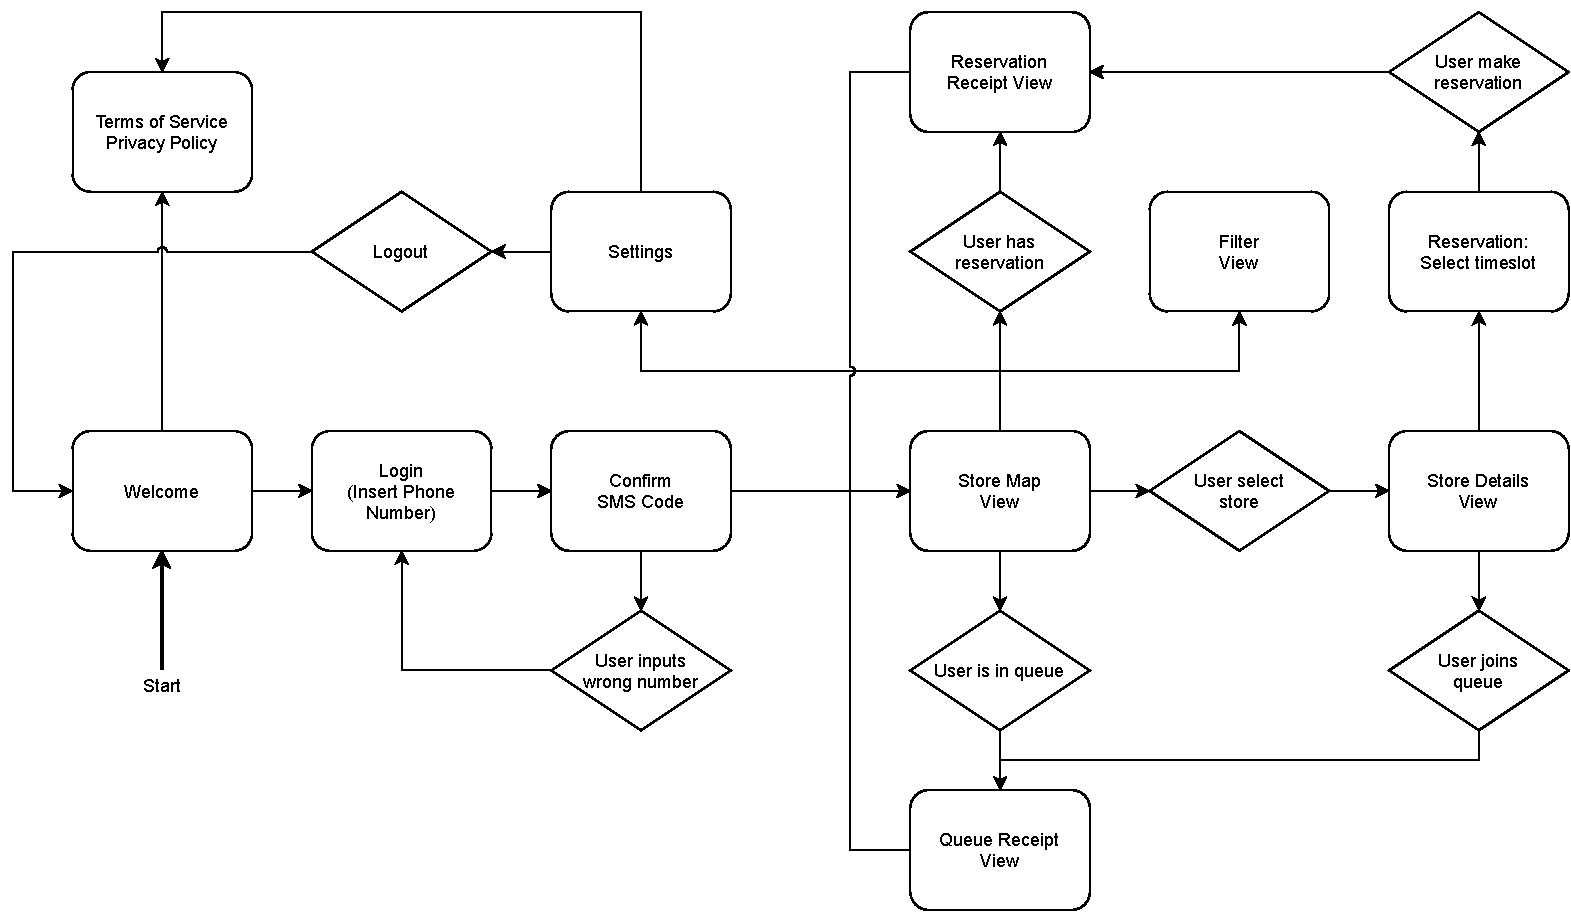
\includegraphics[width=\linewidth]{images/draw.io/ux_diagram.pdf}
    \caption{UX flowchart of the web and mobile application}
    \label{fig:ux_flowchart}
\end{figure}

Additional details can be found in \emph{Section 3.1.1} of the \emph{RASD}.
In the flowchart there are additional views such as a setting page or a viewer for the \emph{Terms of Service} document that don't really need a mockup.

Users need to login in order to use the application, and the can logout through the settings page.

The web application interface will be mostly identical to the mobile application one, in order to provide a coherent experience.

\subsection{Totem application}

The totem interface allows two functionalities: customers can create a ticket for the standard queue, and store employees can authenticate to create a priority queue ticket for a customer.

\begin{figure}[H]
    \centering
    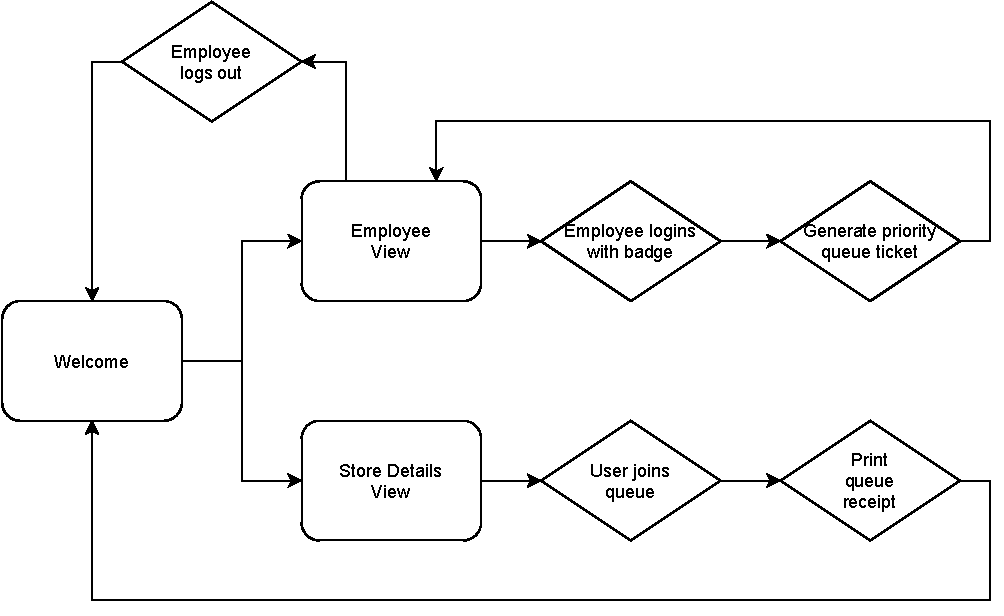
\includegraphics[width=.5\linewidth]{images/draw.io/ux_totem.pdf}
    \caption{UX flowchart of the totem interface}
    \label{fig:ux_totem}
\end{figure}

\subsection{Manager control panel}

The admin web panel allows store managers to add, edit and remove stores.
They need to login beforehand with credentials generated at deployment time.
Managers can edit store details, timeslots, number of allowed customers, and view statistics about stores and users. The hierarchy of the views is illustrated in Fig. \ref{fig:ux_manager_hierarchy}, while the flow and main features of the application is explained in Fig. \ref{fig:ux_manager_flowchart}.

\begin{figure}[H]
    \centering
    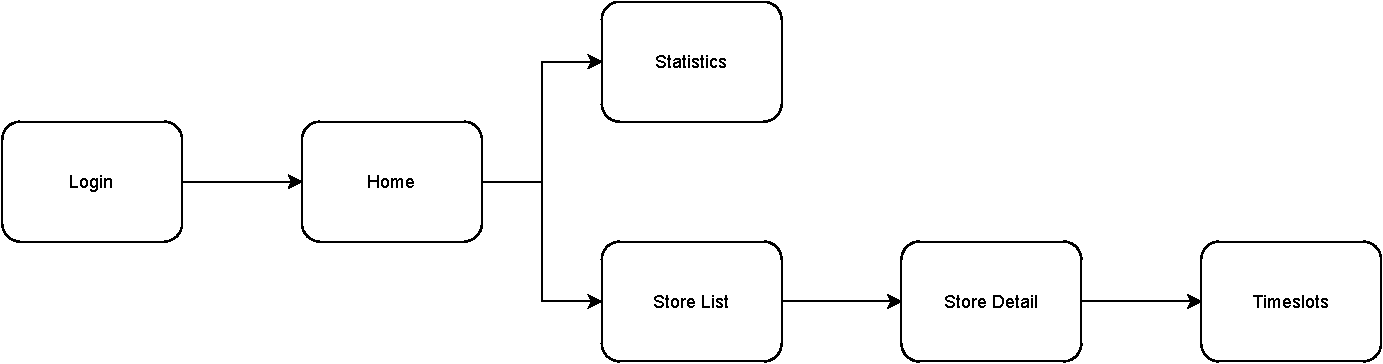
\includegraphics[width=\linewidth]{images/draw.io/ux_manager.pdf}
    \caption{UX hierarchy of manager web panel}
    \label{fig:ux_manager_hierarchy}
\end{figure}

\begin{figure}[H]
    \centering
    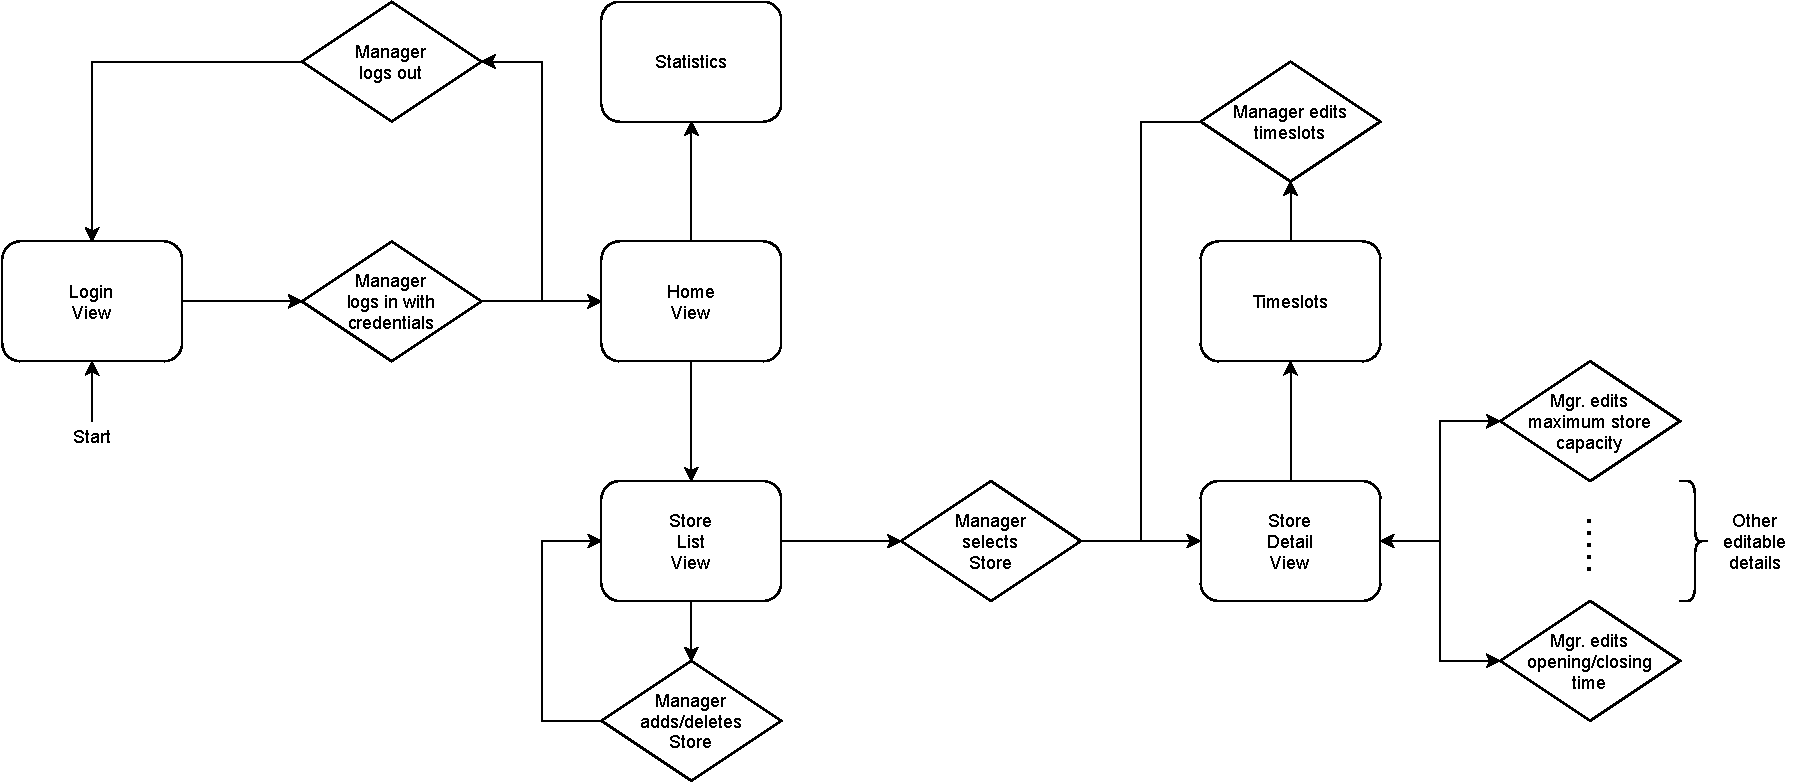
\includegraphics[width=\linewidth]{images/draw.io/ux_manager_flowchart.pdf}
    \caption{UX flowchart of manager web panel}
    \label{fig:ux_manager_flowchart}
\end{figure}